\documentclass{standalone}
\usepackage{tikz}
\usetikzlibrary{patterns, positioning}

\begin{document}
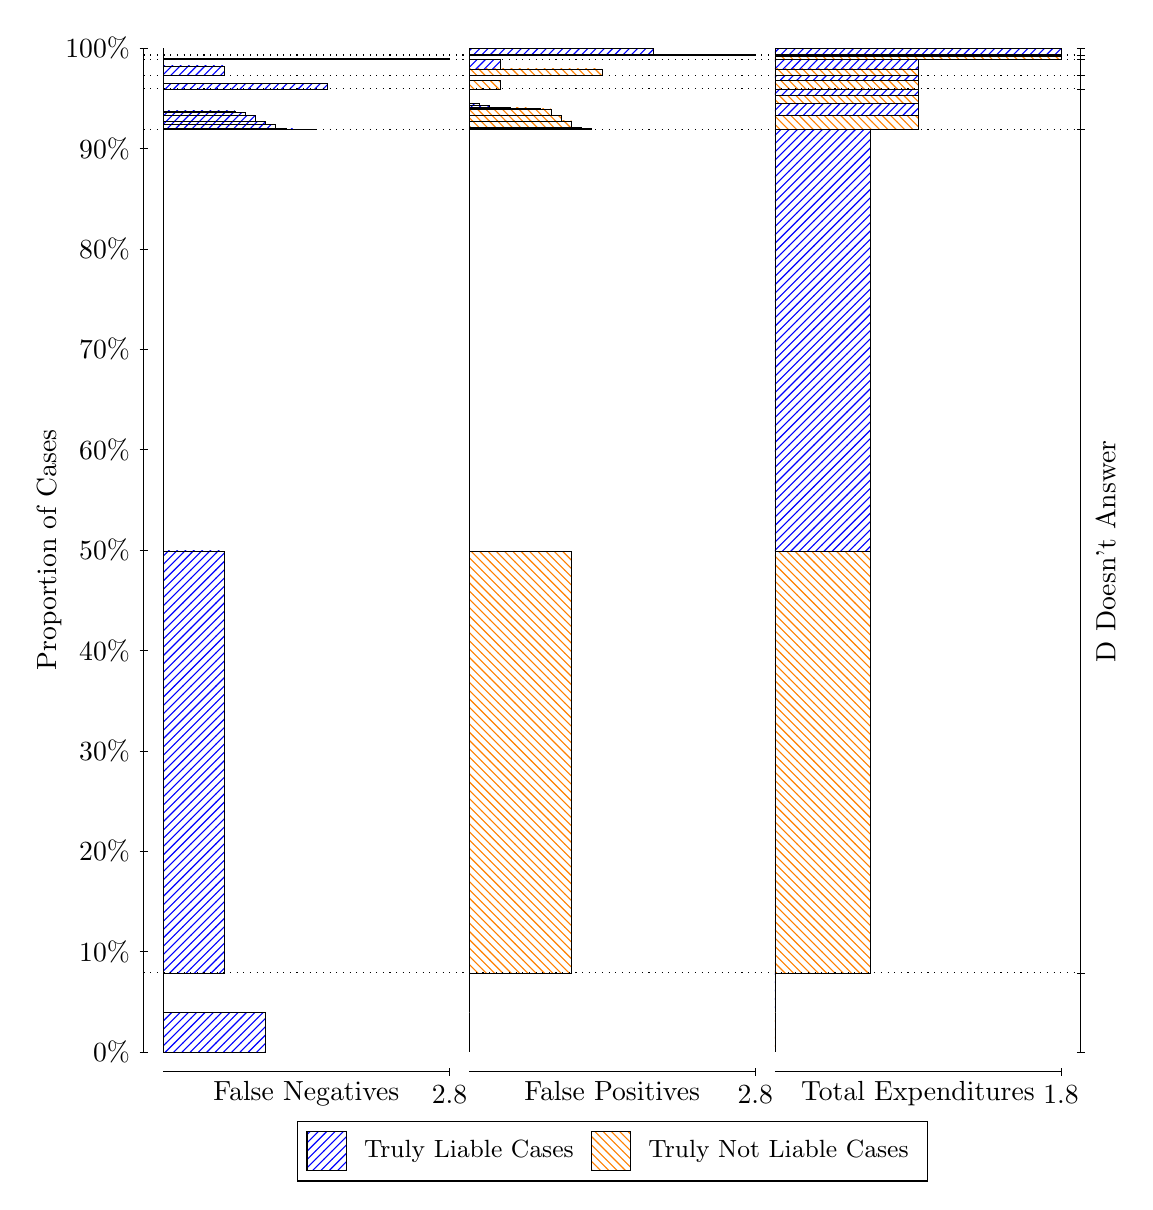
\begin{tikzpicture}
\draw[black, very thin] (1.5,1.75) -- (1.5,14.5);
\node[rotate=90, anchor=center] at (0.3, 8.125) {Proportion of Cases};
\draw[black, very thin] (1.45,1.75) -- (1.55,1.75);
\node[anchor=east] at (1.45, 1.75) {0\%};
\draw[black, very thin] (1.45,3.025) -- (1.55,3.025);
\node[anchor=east] at (1.45, 3.025) {10\%};
\draw[black, very thin] (1.45,4.3) -- (1.55,4.3);
\node[anchor=east] at (1.45, 4.3) {20\%};
\draw[black, very thin] (1.45,5.575) -- (1.55,5.575);
\node[anchor=east] at (1.45, 5.575) {30\%};
\draw[black, very thin] (1.45,6.85) -- (1.55,6.85);
\node[anchor=east] at (1.45, 6.85) {40\%};
\draw[black, very thin] (1.45,8.125) -- (1.55,8.125);
\node[anchor=east] at (1.45, 8.125) {50\%};
\draw[black, very thin] (1.45,9.4) -- (1.55,9.4);
\node[anchor=east] at (1.45, 9.4) {60\%};
\draw[black, very thin] (1.45,10.675) -- (1.55,10.675);
\node[anchor=east] at (1.45, 10.675) {70\%};
\draw[black, very thin] (1.45,11.95) -- (1.55,11.95);
\node[anchor=east] at (1.45, 11.95) {80\%};
\draw[black, very thin] (1.45,13.225) -- (1.55,13.225);
\node[anchor=east] at (1.45, 13.225) {90\%};
\draw[black, very thin] (1.45,14.5) -- (1.55,14.5);
\node[anchor=east] at (1.45, 14.5) {100\%};

\draw[black, very thin] (13.4,1.75) -- (13.4,14.5);
\draw[black, very thin] (13.35,1.75) -- (13.45,1.75);
\node[anchor=west] at (13.35, 1.75) {};
\draw[black, very thin] (13.35,2.754) -- (13.45,2.754);
\node[anchor=west] at (13.35, 2.754) {};
\draw[black, very thin] (13.35,13.463) -- (13.45,13.463);
\node[anchor=west] at (13.35, 13.463) {};
\draw[black, very thin] (13.35,13.982) -- (13.45,13.982);
\node[anchor=west] at (13.35, 13.982) {};
\draw[black, very thin] (13.35,14.151) -- (13.45,14.151);
\node[anchor=west] at (13.35, 14.151) {};
\draw[black, very thin] (13.35,14.356) -- (13.45,14.356);
\node[anchor=west] at (13.35, 14.356) {};
\draw[black, very thin] (13.35,14.411) -- (13.45,14.411);
\node[anchor=west] at (13.35, 14.411) {};
\draw[black, very thin] (13.35,14.5) -- (13.45,14.5);
\node[anchor=west] at (13.35, 14.5) {};

\draw[black, very thin, pattern color=blue, pattern=north east lines] (1.75,1.75) rectangle (3.0476,2.252);
\draw[black, very thin, pattern color=orange, pattern=north west lines] (1.75,2.252) rectangle (1.75,2.754);
\draw[black, very thin, pattern color=blue, pattern=north east lines] (1.75,2.754) rectangle (2.5286,8.1143);
\draw[black, very thin, pattern color=orange, pattern=north west lines] (1.75,8.1143) rectangle (1.75,13.463);
\draw[black, very thin, pattern color=blue, pattern=north east lines] (1.75,13.463) rectangle (3.6964,13.466);
\draw[black, very thin, pattern color=blue, pattern=north east lines] (1.75,13.466) rectangle (3.5667,13.468);
\draw[black, very thin, pattern color=blue, pattern=north east lines] (1.75,13.468) rectangle (3.4369,13.474);
\draw[black, very thin, pattern color=blue, pattern=north east lines] (1.75,13.474) rectangle (3.3071,13.48);
\draw[black, very thin, pattern color=blue, pattern=north east lines] (1.75,13.48) rectangle (3.1774,13.526);
\draw[black, very thin, pattern color=blue, pattern=north east lines] (1.75,13.526) rectangle (3.0476,13.573);
\draw[black, very thin, pattern color=blue, pattern=north east lines] (1.75,13.573) rectangle (2.9179,13.647);
\draw[black, very thin, pattern color=blue, pattern=north east lines] (1.75,13.647) rectangle (2.7881,13.678);
\draw[black, very thin, pattern color=blue, pattern=north east lines] (1.75,13.678) rectangle (2.6583,13.702);
\draw[black, very thin, pattern color=orange, pattern=north west lines] (1.75,13.702) rectangle (1.75,13.982);
\draw[black, very thin, pattern color=blue, pattern=north east lines] (1.75,13.982) rectangle (3.8262,14.047);
\draw[black, very thin, pattern color=orange, pattern=north west lines] (1.75,14.047) rectangle (1.75,14.151);
\draw[black, very thin, pattern color=blue, pattern=north east lines] (1.75,14.151) rectangle (2.5286,14.272);
\draw[black, very thin, pattern color=orange, pattern=north west lines] (1.75,14.272) rectangle (1.75,14.356);
\draw[black, very thin, pattern color=blue, pattern=north east lines] (1.75,14.356) rectangle (5.3833,14.369);
\draw[black, very thin, pattern color=orange, pattern=north west lines] (1.75,14.369) rectangle (1.75,14.411);
\draw[black, very thin, pattern color=orange, pattern=north west lines] (1.75,14.411) rectangle (1.75,14.424);
\draw[black, very thin, pattern color=blue, pattern=north east lines] (1.75,14.424) rectangle (1.75,14.5);
\draw[black, very thin, pattern color=orange, pattern=north west lines] (5.6333,1.75) rectangle (5.6333,2.252);
\draw[black, very thin, pattern color=blue, pattern=north east lines] (5.6333,2.252) rectangle (5.6333,2.754);
\draw[black, very thin, pattern color=orange, pattern=north west lines] (5.6333,2.754) rectangle (6.931,8.1029);
\draw[black, very thin, pattern color=blue, pattern=north east lines] (5.6333,8.1029) rectangle (5.6333,13.463);
\draw[black, very thin, pattern color=orange, pattern=north west lines] (5.6333,13.463) rectangle (7.1905,13.478);
\draw[black, very thin, pattern color=orange, pattern=north west lines] (5.6333,13.478) rectangle (7.0607,13.494);
\draw[black, very thin, pattern color=orange, pattern=north west lines] (5.6333,13.494) rectangle (6.931,13.575);
\draw[black, very thin, pattern color=orange, pattern=north west lines] (5.6333,13.575) rectangle (6.8012,13.649);
\draw[black, very thin, pattern color=orange, pattern=north west lines] (5.6333,13.649) rectangle (6.6714,13.728);
\draw[black, very thin, pattern color=orange, pattern=north west lines] (5.6333,13.728) rectangle (6.5417,13.734);
\draw[black, very thin, pattern color=orange, pattern=north west lines] (5.6333,13.734) rectangle (6.4119,13.739);
\draw[black, very thin, pattern color=orange, pattern=north west lines] (5.6333,13.739) rectangle (6.2821,13.741);
\draw[black, very thin, pattern color=orange, pattern=north west lines] (5.6333,13.741) rectangle (6.1524,13.744);
\draw[black, very thin, pattern color=blue, pattern=north east lines] (5.6333,13.744) rectangle (5.8929,13.767);
\draw[black, very thin, pattern color=blue, pattern=north east lines] (5.6333,13.767) rectangle (5.7631,13.798);
\draw[black, very thin, pattern color=blue, pattern=north east lines] (5.6333,13.798) rectangle (5.6333,13.982);
\draw[black, very thin, pattern color=orange, pattern=north west lines] (5.6333,13.982) rectangle (6.0226,14.086);
\draw[black, very thin, pattern color=blue, pattern=north east lines] (5.6333,14.086) rectangle (5.6333,14.151);
\draw[black, very thin, pattern color=orange, pattern=north west lines] (5.6333,14.151) rectangle (7.3202,14.236);
\draw[black, very thin, pattern color=blue, pattern=north east lines] (5.6333,14.236) rectangle (6.0226,14.356);
\draw[black, very thin, pattern color=orange, pattern=north west lines] (5.6333,14.356) rectangle (5.6333,14.398);
\draw[black, very thin, pattern color=blue, pattern=north east lines] (5.6333,14.398) rectangle (5.6333,14.411);
\draw[black, very thin, pattern color=orange, pattern=north west lines] (5.6333,14.411) rectangle (9.2667,14.424);
\draw[black, very thin, pattern color=blue, pattern=north east lines] (5.6333,14.424) rectangle (7.969,14.5);
\draw[black, very thin, pattern color=orange, pattern=north west lines] (9.5167,1.75) rectangle (9.5167,2.252);
\draw[black, very thin, pattern color=blue, pattern=north east lines] (9.5167,2.252) rectangle (9.5167,2.754);
\draw[black, very thin, pattern color=orange, pattern=north west lines] (9.5167,2.754) rectangle (10.728,8.1029);
\draw[black, very thin, pattern color=blue, pattern=north east lines] (9.5167,8.1029) rectangle (10.728,13.463);
\draw[black, very thin, pattern color=orange, pattern=north west lines] (9.5167,13.463) rectangle (11.333,13.641);
\draw[black, very thin, pattern color=blue, pattern=north east lines] (9.5167,13.641) rectangle (11.333,13.795);
\draw[black, very thin, pattern color=orange, pattern=north west lines] (9.5167,13.795) rectangle (11.333,13.897);
\draw[black, very thin, pattern color=blue, pattern=north east lines] (9.5167,13.897) rectangle (11.333,13.982);
\draw[black, very thin, pattern color=orange, pattern=north west lines] (9.5167,13.982) rectangle (11.333,14.086);
\draw[black, very thin, pattern color=blue, pattern=north east lines] (9.5167,14.086) rectangle (11.333,14.151);
\draw[black, very thin, pattern color=orange, pattern=north west lines] (9.5167,14.151) rectangle (11.333,14.236);
\draw[black, very thin, pattern color=blue, pattern=north east lines] (9.5167,14.236) rectangle (11.333,14.356);
\draw[black, very thin, pattern color=orange, pattern=north west lines] (9.5167,14.356) rectangle (13.15,14.398);
\draw[black, very thin, pattern color=blue, pattern=north east lines] (9.5167,14.398) rectangle (13.15,14.411);
\draw[black, very thin, pattern color=orange, pattern=north west lines] (9.5167,14.411) rectangle (13.15,14.424);
\draw[black, very thin, pattern color=blue, pattern=north east lines] (9.5167,14.424) rectangle (13.15,14.5);
\draw[black, dotted] (1.5,2.754) -- (13.4,2.754);
\draw[black, dotted] (1.5,13.463) -- (13.4,13.463);
\draw[black, dotted] (1.5,13.982) -- (13.4,13.982);
\draw[black, dotted] (1.5,14.151) -- (13.4,14.151);
\draw[black, dotted] (1.5,14.356) -- (13.4,14.356);
\draw[black, dotted] (1.5,14.411) -- (13.4,14.411);
\draw[black, very thin] (1.75,1.5) -- (5.3833,1.5);
\node[anchor=north] at (3.5667, 1.5) {False Negatives};
\draw[black, very thin] (5.3833,1.45) -- (5.3833,1.55);
\node[anchor=north] at (5.3833, 1.45) {2.8};

\draw[black, very thin] (5.6333,1.5) -- (9.2667,1.5);
\node[anchor=north] at (7.45, 1.5) {False Positives};
\draw[black, very thin] (9.2667,1.45) -- (9.2667,1.55);
\node[anchor=north] at (9.2667, 1.45) {2.8};

\draw[black, very thin] (9.5167,1.5) -- (13.15,1.5);
\node[anchor=north] at (11.333, 1.5) {Total Expenditures};
\draw[black, very thin] (13.15,1.45) -- (13.15,1.55);
\node[anchor=north] at (13.15, 1.45) {1.8};


\node[black, centered, rotate=90] at (13.72, 8.1086) {D Doesn't Answer};






\draw (7.449999999999999,1.5) node[draw=none] (baseCoordinate) {};
\begin{scope}[align=center]
        \matrix[scale=0.5, draw=black, below=0.5cm of baseCoordinate, nodes={draw}, column sep=0.1cm]{
            \node[rectangle, draw, minimum width=0.5cm, minimum height=0.5cm, pattern=north east lines, pattern color=blue] {}; &
            \node[draw=none, font=\small] (B) {Truly Liable Cases}; &
            \node[rectangle, draw, minimum width=0.5cm, minimum height=0.5cm, pattern=north west lines, pattern color=orange] {}; &
            \node[draw=none, font=\small] (B) {Truly Not Liable Cases}; \\
            };
\end{scope}

\end{tikzpicture}
\end{document}